% !TEX root = ../../../main.tex
% 来源：高中物理甲种本·第一册（力学）
% 章节：运动定律 / 牛顿运动定律的适用范围
% 原始文件：3.tex，行 1117-1124
% 类型：tikz
% ---
    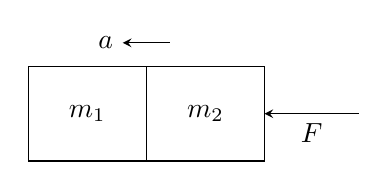
\begin{tikzpicture}[scale=.6, >=stealth]
       \draw  (0,0) rectangle (5, 2);
       \draw  (0,0) rectangle (2.5, 2);
    \node at (2.5/2,1){$m_1$};
    \node at (2.5+2.5/2,1){$m_2$};
    \draw[<-](5,1)--node [below]{$F$}(7,1);
    \draw[<-](2,2.5)node [left]{$a$}--(3,2.5);
    \end{tikzpicture}
